\begin{exsol}{10}{Cabral 7.6 Hernan Cortez}{180}{Foundations}{B2}
\asked Explain the strategic value of Cort\'es sinking his own ships on arrival in Mexico, given
that his force expected resistance from the native population.

\method Sequential games, backward induction and the value of credible commitment (Cabral
\S7.2, pp.~167--171, Figures 7.7--7.9: a player gains by removing or penalizing its own options).
Course link: \MR{} on achieving commitment, where William the Conqueror and Cort\'es are the
examples (Ch.~5, pp.~133, 139; notes, Aula~2, ``Commitment, reputation and the ultimatum
game'').

\solution
\subparagraph{(a) The game without commitment.} Model the Cabral entry game of Figure~7.7 with
the roles adapted. The natives (N) move first: resist (R) or not (NR). If they resist, the
Spaniards (S) choose to fight (F) or leave by sea (L). Illustrative payoffs (N, S), chosen only
to respect the ordering of the story:
\begin{center}
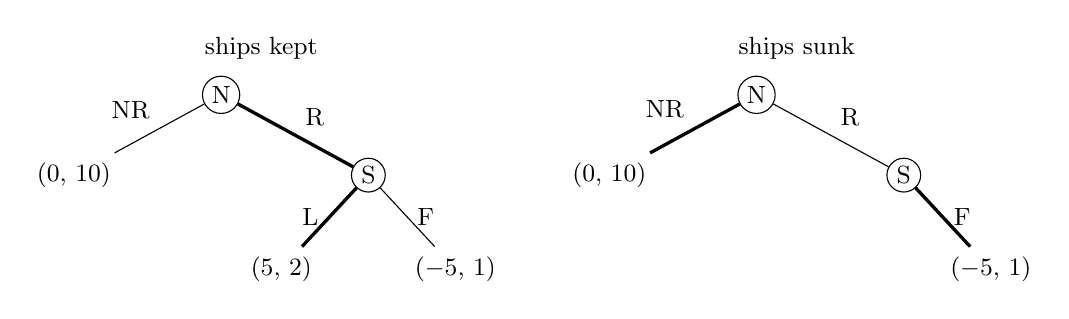
\begin{tikzpicture}[scale=0.85, every node/.style={font=\small},
  dec/.style={circle,draw,inner sep=1.5pt}]
  \node[dec] (n) at (0,0) {N};
  \node[dec] (s) at (2.2,-1.2) {S};
  \node (nr) at (-2.2,-1.2) {$(0,\,10)$};
  \node (l) at (0.9,-2.6) {$(5,\,2)$};
  \node (f) at (3.5,-2.6) {$(-5,\,1)$};
  \draw (n) -- node[above left] {NR} (nr);
  \draw (n) -- node[above right] {R} (s);
  \draw[very thick] (s) -- node[left] {L} (l);
  \draw (s) -- node[right] {F} (f);
  \draw[very thick] (n) -- (s);
  \node at (0.6,0.7) {ships kept};
  \begin{scope}[xshift=8cm]
  \node[dec] (n2) at (0,0) {N};
  \node[dec] (s2) at (2.2,-1.2) {S};
  \node (nr2) at (-2.2,-1.2) {$(0,\,10)$};
  \node (f2) at (3.5,-2.6) {$(-5,\,1)$};
  \draw[very thick] (n2) -- node[above left] {NR} (nr2);
  \draw (n2) -- node[above right] {R} (s2);
  \draw[very thick] (s2) -- node[right] {F} (f2);
  \node at (0.6,0.7) {ships sunk};
  \end{scope}
\end{tikzpicture}
\end{center}
Not resisting hands the Spaniards the full prize ($10$); a resisted campaign that ends in
withdrawal leaves them with little ($2$) and the natives better off ($5$); a fought war is costly
for both ($-5$, $1$). Backward induction (thick branches): if resisted, the Spaniards compare
$2$ (leave) with $1$ (fight) and leave. The natives anticipate this and compare $5$ (resist) with
$0$ (not resist), so they resist. Outcome: $(5,2)$. The Spaniards' threat to fight to the end is
not credible, exactly like the incumbent's threat in Figure~7.7 (p.~169).

\subparagraph{(b) Sinking the ships.} Destroying the fleet deletes the branch L. Now a resisted
Spaniard can only fight, so resisting gives the natives $-5 < 0$ and they do not resist.
Outcome: $(0,10)$. The value of commitment is $10 - 2 = 8$ for the Spaniards, and the move is
worth making whenever the ships' value is below $8$. This is Cabral's bond of Figure~7.8 taken to
the limit: instead of a penalty for retreating, retreat becomes impossible (equivalently, the
Spaniards now move first, as in Figure~7.9, p.~171).

\subparagraph{(c) Two audiences.} The quotation itself (``I could act more securely'') stresses
a second effect. Before the ships were sunk, any of Cort\'es's own men could press to go back;
afterwards no one could, so each soldier's best response changed from hedging to fighting
hard. The same commitment therefore works on the rival (it changes what the natives expect the
Spaniards to do) and inside the organization (it removes an exit option, aligning the members'
interests with the leader's plan).

\subparagraph{(d) Conditions and costs.} Commitment has value only if (i) it is irreversible:
a fleet that can be refloated commits nothing; (ii) the other side observes it, since a
commitment no one knows about cannot change their choice; and (iii) the cost is accepted: \MR{}
note that such noncontractual commitments ``may be worthwhile, but costly'', since the fleets
were perfectly good (p.~139). If the natives resist anyway (they did not see the act, or misread
it), the Spaniards are stuck with $1$ instead of the $2$ they could have had by leaving.

\interp Bargaining power comes from what a player can credibly do next, and a player can raise
its power by \emph{reducing} its own options. The same logic runs through the course: the
proposer in an ultimatum game is committed to walking away, specialized investments commit a
firm to a strategy (Apple's Macintosh plant, \MR{} p.~133), and the hold-up problem of item~30 is
the reverse case, where a sunk investment weakens the investor's position.

\verify The script \texttt{check\_B.py} solves both trees by backward induction: $(5,2)$ with the
ships, $(0,10)$ without, a commitment value of $8$. Robustness: the result needs only the
orderings $u_S(\text{leave}) > u_S(\text{fight})$, $u_N(\text{resist, leave}) > u_N(\text{no
resistance}) > u_N(\text{resist, fight})$ and $u_S(\text{no resistance}) >
u_S(\text{resist, leave})$; any payoffs with these orderings give the same two equilibria.

\answer{Sinking the ships was a credible commitment. With the fleet available, a resisted
Spaniard would rather leave than fight, so resistance pays and the natives resist. Without
it, the only option is to fight, which makes resistance unprofitable and (in the model) deters
it; it also
stops Cort\'es's own men from hedging. The move is valuable only because it is irreversible,
observed and costly, as in Cabral \S7.2 (pp.~169--171).}
\end{exsol}
